%! Author = lazza
%! Date = 06/05/2022

\section{HW speculation}\label{sec:hw-speculation}
HW-based speculation combines three ideas:
\begin{description}[noitemsep]
    \item[Dynamic Branch Prediction] to choose which instruction to execute
    \item[Dynamic Scheduling] supporting out-of-order execution but in-order commit to prevent any irrevocable
    actions (such as register update or taking exception) until an instruction commits
    \item[Speculation] To execute instructions before control dependencies are solved
\end{description}
The idea is allowing instruction to execute freely and out-of-order, based on speculation, but allow to update the RF
or the memory only when an instruction is no longer speculative.

Mechanisms are necessary to handle incorrect speculation, hardware speculation extends dynamic scheduling beyond a
branch, i.e., behind the basic blocks.

\subsection{Reorder buffer}\label{subsec:reorder-buffer}
A buffer that holds instruction results before they are committed.
When an instruction complete execution, the results are placed into ROB, which holds the instructions in FIFO order,
exactly as issued.
The result in the ROB buffer are tagged, they are used instead of the reservation stations, supplying operands to
other instruction between execution and commit.
The instruction at the \textbf{head} of ROB can safely commit, all its predecessor have already committed.

\begin{figure}[h]
    \centering
    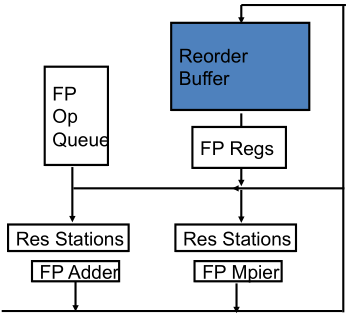
\includegraphics[scale = 0.4]{images/reorder-buffer}
    \caption{ROB}
    \label{fig:rob}
\end{figure}

\paragraph{Separating Completion from Commit} Re-order buffer holds the register result from completion until commit:
\begin{itemize}[noitemsep]
    \item[-] entries are allocated in program order during decode
    \item[-] it buffers completed values and exception state until commit point
    \item[-] completed values can be used by dependents before committed (bypassing)
    \item[-] each entry holds a program counter, instruction type, destination register specifier and value if any,
    and exception status
\end{itemize}

\paragraph{Memory reordering} It needs special data structures:
speculative store address and data buffers, speculative load address and data buffers.

\paragraph{Precise interrupts and Speculation} If a speculation is wrong, we need to be able to back and restart
execution to a point before out incorrect prediction (e.g., branch prediction), it happens the same as precise
exceptions.
The recovery technique for both is \textbf{in-order commit}.


\subsection{Speculative Tomasulo}\label{subsec:speculative-tomasulo}
\subsubsection{Stages}
\begin{description}
    \item[Issue] get instruction from FP Op Queue.\\
    If the reservation station \textcolor{red}{and reorder buffer slot} are free: issue instruction, send
    operands, \textcolor{red}{reorder buffer number for destination.}
    \item[Execution] operate on operands when ready.\\
    If not ready, watch CDB for result: when both are in the reservation station, execute then check for RAW.
    \item[Write result] finish execution.\\
    Write on Common Data Bus to all awaiting FUs \textcolor{red}{and reorder buffer}.
    Mark the reservation station available.
    \item[Commit] \textcolor{red}{update register with reorder result}.\\
    \textcolor{red}{When and instruction at the head of ROB and the result is present, update the register or memory,
        and remove instruction from ROB. In case of mispredicted branch flush the reorder buffer.}\\
    Three types of commit:
    \begin{itemize}[noitemsep]
        \item normal commit
        \item store commit
        \item flush results if incorrect branch prediction
    \end{itemize}
\end{description}

\begin{figure}
    \centering
    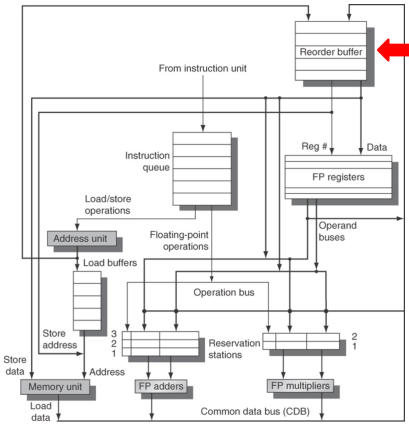
\includegraphics[scale = 0.5]{images/speculative-tomasulo}
    \caption{Speculative tomasulo}
    \label{fig:speculative-tomasulo}
\end{figure}

\subsubsection{ROB entries}
Each ROB entries contains four fields:
\begin{description}
    \item[Instruction type field] indicates whether instruction
    is a branch (no destination result), a store (has
    memory address destination), or a load/ALU
    (register destination)
    \item[Destination field] supplies register number (for
    loads and ALU instructions) or memory address (for
    stores) where results should be written
    \item[Value field] holds value of result until
    instruction commits
    \item[Ready filed] indicates that instruction has
    completed execution, ready to commit
\end{description}

\subsubsection{ROB extension}
The addition of the reorder buffer introduces changes in tomasulo:
\begin{itemize}[noitemsep]
    \item ROB completely replaces store buffers
    \item renaming function of reservation stations completely replaced
    \item reservation stations now only queue operations (and operands) to FUs between issue and execution.
    \item results are tagged with ROB entry number rather than with RS number, ROB entry must be tracked in the
    reservation stations
    \item all instructions excluding incorrectly predicted branches (or incorrectly speculated loads) commit when
    reaching head of ROB
    \item when a incorrectly predicted branch reaches the head, ROB is flushed, execution restarts at correct
    successor of branch \textrightarrow speculative active are easily undone
    \item processor with ROB can dynamically speculate while maintaining a precise interrupt model
\end{itemize}

